\chapter{Implementación}

La implementación de este proyecto se ha llevado a cabo en dos fases diferenciadas: la creación del sistema experto y el desarrollo de la aplicación web,utilizada como interfaz, en la que será embebido. 

Todo el código puede ser consultado en \cite{CODIGO}.

\section{Sistema experto}

El primer paso fue la creación de un prototipo utilizando el entorno de CLIPS. A continuación, se explican las decisiones tomadas a lo largo del desarrollo de este prototipo.

\subsection{Formato de los datos de entrada: partitura}

Una de las primeras cuestiones fue cómo obtener la información necesaria del XML en el que está contenida la partitura. Dado que CLIPS no puede procesar el XML para leer el contenido de las etiquetas, está funcionalidad tenía que ser realizada por Python. Sin embargo, definimos las estructuras que debían tener los ficheros para poder ser leídos por CLIPS y añadir esa información en forma de hechos.

Los datos que teníamos que extraer de la partitura eran:

\begin{itemize}

	\item La \textbf{tonalidad} de la obra. La tonalidad es la que nos define la \textit{escala musical} sobre la que está construido el coral. Nos da la relación entre los acordes y sus funciones tonales. La tonalidad está compuesta por el nombre y el modo.

	\item El \textbf{compás}. El compás nos indica cuántas figuras de un determinado tipo hay en cada pulso. El compás está compuesto por dos números que nos indican el número de pulsos y el tipo de figura que dura un pulso:

	\begin{itemize}
		\item 1: redonda
		\item 2: blanca
		\item 4: negra
		\item 8: corchea
	\end{itemize}

	\item Las \textbf{notas} de cada voz. Las notas musicales vienen definidas por su nombre, su altura, su duración y su alteración.

	\item Los \textbf{movimientos} de cada voz. Los movimientos nos indican si la voz, de una nota a otra, se mueve de forma ascendente, descendente o se mantiene.

\end{itemize}

Para cada uno de estos datos se creo una plantilla con la instrucción ``\texttt{deftemplate}'', al igual que para el resto de hechos como se mencionó en el capítulo \textit{Adquisición de conocimientos}. 

\subsubsection{Estructura del archivo de notas}

Una de las mayores dificultades fue decidir la estructura del archivo que contendría la información sobre las notas. Cada nota tiene una duración independiente, lo cual a la hora de realizar el análisis armónico resulta muy complejo. Al analizar la armonía de una obra tenemos que tener en cuenta todas las voces al mismo tiempo, analizamos de forma vertical. Sin embargo, en una misma parte cada nota de cada voz puede tener una duración distinta y por ende puede formarse más de un acorde en dicha parte. Esto significa que no siempre va a haber el mismo número de acordes, ni de notas, en cada compás.

En la práctica, a un experto este hecho no le resulta un problema, porque puede observar las voces gráficamente y poder determinar cuándo termina la duración de cada nota y el acorde. En cambio, para un sistema experto, al no saber dónde termina cada nota con respecto a las demás, no puede hacer esas deducciones de manera tan sencilla. 

Para solucionar este problema, decidí subdividir todas las notas de todas las voces a semicorcheas, que es la figura musical más pequeña que se suele utilizar en los corales. De esta forma, conseguimos que en todos los compases haya el mismo número de notas en cada voz.

En la siguiente figura, se muestra gráficamente lo que supone esta transformación:


\begin{figure}[H]
	\centering
	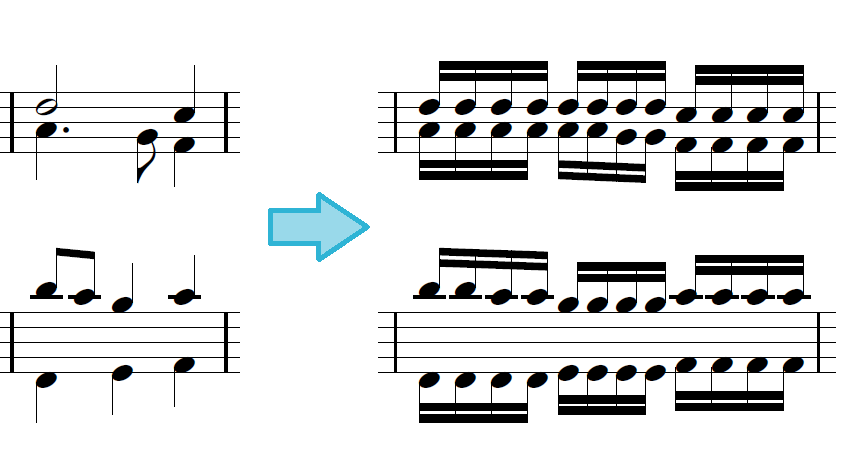
\includegraphics[scale=0.5]{imagenes/division.png}
	\caption{Subdivisión de un compás del coral ``Aus meines Herzens Grunde'' de \textit{J.S.Bach} a semicorcheas}
	\label{fig5.1.1}
\end{figure}

Como podemos ver, al realizar esta subdivisión podemos ir analizando en bloques equivalente en tiempo. Los resultados del análisis no se ven afectados, dado que únicamente hemos modificado la duración de las notas, la cual no interviene en los errores que vamos a detectar.

En el caso del análisis melódico, no es necesario hacer esta subdivisión porque analizamos cada voz de manera independientede de las otras, analizamos la partitura horizontalmente.

\subsubsection{Formatos finales}

Las estructuras de los ficheros que leería el sistema experto quedarían de la siguiente manera:

\begin{itemize}

	\item Fichero de la tonalidad:

		\begin{lstlisting}[frame=single]

			Nombre Modo

		\end{lstlisting}

		Ejemplo:

		\begin{lstlisting}[frame=single]

			D Mayor

		\end{lstlisting} 

	\bigskip
	\item Fichero del compás:

		\begin{lstlisting}[frame=single]

			Partes Figura

		\end{lstlisting}

		Ejemplo:

		\begin{lstlisting}[frame=single]

			3 4

		\end{lstlisting} 

	\bigskip
	\item Fichero de notas: se crearía un fichero para cada voz.
	
		\begin{lstlisting}[frame=single]

			Nombre Alteracion Altura Nombre Alteracion Altura ...

		\end{lstlisting} 

		Ejemplo:

		\begin{lstlisting}[frame=single]

			A b 4 B 2 D s 3

		\end{lstlisting} 

	\bigskip
	\item Movimientos:

		\begin{lstlisting}[frame=single]

			Movimiento1 Movimiento2 Movimiento3 ...

		\end{lstlisting} 

		Ejemplo:

		\begin{lstlisting}[frame=single]

			Ascendente Ascendente Descendente

		\end{lstlisting} 

\end{itemize}

Los nombres de las notas se representarán con el cifrado americano, el empleado en el archivo XML. La equivalencia entre el cifrado americano y el empleado en occidente es:

\begin{itemize}

	\item Do $\rightarrow$ C
	\item Re $\rightarrow$ D
	\item Mi $\rightarrow$ E
	\item Fa $\rightarrow$ F
	\item Sol $\rightarrow$ G
	\item La $\rightarrow$ A
	\item Si $\rightarrow$ B

\end{itemize}

\subsection{Implementación del primer prototipo}

En el primer prototipo, no se modularizaron los hechos y reglas en función de los módulos descritos en los capítulos anteriores. Esto es porque aún no estaban definidas del todo las dependencias de las reglas respecto a los hechos ni la división del análisis armónico en dos partes realmente diferenciadas. 

Aunque en el análisis y el diseño quedan claras estas divisiones, a la hora de implementar las reglas, iban surgiendo muchas relaciones entre todos los hechos de la base de conocimiento. Por ejemplo, se esperaba que los hechos referidos a los movimientos de las voces únicamente fueran utilizados por el módulo del análisis melódico. Sin embargo, también es necesario para localizar algunos errores armónicos. Además, la existencia de algunos errores melódicos provoca a su vez errores armónicos y viceversa. 

Una vez se terminaron de implementar todas las reglas y hechos, se procedió a verificar y validar el prototipo. 

La  \textbf{verificación} consistió en comprobar que los ficheros se leían correctamente y los hechos deducidos se asertaban en el sistema de la manera esperada. Esto se comprobó fácilmente observando la ventana de hechos que aparece en la propia interfaz de CLIPS.

La \textbf{validación} se realizó creando archivos de prueba, con los formatos descritos anteriormente, que contuviesen al menos un error de cada tipo. Los modelos de prueba fueron recogidos de las fuentes bibliográficas, las cuáles contienen una gran cantidad de ejemplos

\subsection{Modularización del sistema}

Tras la creación del primer prototipo y su verificación y validación, comencé el proceso de modularización del sistema. 

Al estar implementadas todas las reglas y funcionalidades del sistema, este proceso, aunque tedioso, fue el más sencillo. 

Fui comprobando para cada regla los antencendentes que debían cumplirse y así poder agruparlas según los hechos que necesitaban.
Una vez agrupadas, pude definir los hechos asertados necesarios para cada uno de los módulos.

Como resultado final, obtuve los tres módulos de análisis, cada uno con sus reglas y hechos diferenciados. 

\section{Aplicación web}

La implementación de la aplicación web, como se comentó en el capítulo anterior, se ha hecho utilizando el framework DJango de Python.

La finalidad de implementar esta aplicación es proporcionar al sistema experto una interfaz agradable y sencilla de utilizar para el usuario. 

Este portal se encargará de las siguientes funciones:
\begin{itemize} 
	\item El envío de un formulario con las opciones de análisis seleccionadas por el usuario y el archivo de la partitura a analizar.
	\item La extracción de datos del archivo XML de la partitura y escritura de los mismos en ficheros según se describe en la sección anterior.
	\item La ejecución de los módulos seleccionados del sistema experto.
	\item Mostrar los errores detectados.
\end{itemize}

\subsection{Tratamiento del archivo XML}

Como se ha comentado antes, CLIPS no puede extraer la información de las etiquetas del archivo XML. Esta tarea es implementada por Python haciendo uso de la API \textit{ElementTree XML}. Esta API nos permite buscar etiquetas y leer el contenido de las mismas. 

Los archivos XML que contienen partituras, hacen uso de una gran cantidad de etiquetas. En este caso, para extraer los datos necesarios consultamos las siguientes:

\begin{itemize}

	\item \textit{Key}: para extraer la tonalidad.
	\item \textit{Time}: para extraer el compás.
	\item \textit{Note}: para extraer información de la nota. Dentro de ésta consultamos la siguientes subetiquetas:
		\begin{itemize}
			\item \textit{Pitch}: para extraer el nombre y la octava. 
			\item \textit{Accidental}: para comprobar si tenía una alteración accidental.
			\item \textit{Type} y \textit{Dot}: para extraer la duración.
			\item \textit{Voice}: para extraer la voz que canta dicha nota.
		\end{itemize}
\end{itemize}

La información contenida en las etiquetas se escribe en ficheros de acuerdo al formato que definimos.

\subsubsection{Determinación de movimientos melódicos}

Para el análisis melódico y algunas cuestiones del análisis armónico es necesario conocer la dirección que van tomando las melodías. Esta información no viene representada de forma explícita en el archivo de la partitura, sino que debemos de extraerla nosotros. 

Una vez se han creado los archivos que contienen las notas de las voces, vamos comprobando las notas dos a dos para determinar si la melodía hace un movimiento descendente, ascendente o se mantiene. 

La lista de movimientos de cada voz se escribe en un fichero para ser utilizado por los módulos de análisis.

\subsection{Integración del sistema experto}

Esta fase de la implementación fue la que presentó más problemas. Para integrar el sistema con la interfaz web he utilizado la librería PyCLIPS. Esta librería permite utilizar las funciones de CLIPS para crear sistema expertos en Python. Además, también permite cargar archivos creados en CLIPS y ejecutarlos.

Gracias a esta última característica, en un principio se pensó que únicamente sería necesario cargar los archivos de los módulos y  ejecutarlos cuando fuera necesario. Sin embargo, hubo que hacer algunas modificaciones.

El primer problema con el que me encontré fue que los archivos no podían cargarse. Tras buscar en la documentación de PyCLIPS \cite{PYCLIPS}, encontré la respuesta a este problema. PyCLIPS permite cargar archivos de CLIPS que contengan reglas o hechos, pero no ambas en un mismo fichero. Así pues, dividí los ficheros en ficheros con reglas y ficheros con hechos. 

De nuevo, surgió otro problema, esta vez con los archivos de hechos. En este caso, no se aceptaban las definiciones de las estructuras \texttt{deftemplate}. Para solucionarlo, decidí añadirlas utilizando explícitamente las funciones de PyCLIPS. A pesar de que parecía haberse solucionado, esto derivó en nuevos problemas asociados a dos funciones de CLIPS: las funciones \texttt{clear} y \texttt{reset}.

\bigskip
La función \texttt{clear} borra todo el entorno de CLIPS, eliminando de la memoria de trabajo todos los hechos, reglas, plantillas y funciones que estuviesen definidos.

\bigskip
La función \texttt{reset} reinicia el entorno, eliminando sólo los hechos y dejando en la memoria de trabajo todas las reglas, plantillas y funciones.

\bigskip

Antes de la ejecución de cada módulo se siguen los siguientes pasos:

\begin{itemize}
	\item Se transforma el XML a los archivos de entrada del sistema experto.
	\item Se limpia el entorno.
	\item Se reinicia el entorno.
	\item Se cargan las plantillas del módulo.
	\item Se cargan los hechos del módulo.
	\item Se cargan las reglas del módulo.
\end{itemize}

Debido a algún problema con la librería PyCLIPS o el intérprete de Python, la función \texttt{clear} no puede ejecutarse. Esto provoca que cada vez que se lancen los módulos del sistema, se redefinan las plantillas con las funciones de PyCLIPS. CLIPS no permite sobreescribir hechos o plantillas, por lo que nos daba un error de redefinición. 

Para el correcto funcionamiento del sistema, las plantillas debían ser definidas una única vez al inicio del sistema. Tras consultar la documentación y el foro de la comunidad encontré la solución: había que definir las plantillas en el archivo \texttt{urls.py}. Este archivo contiene las expresiones regulares de las ``urls'' en las que se visualizarán las secciones de la pagina web. Éste código se ejecuta una única vez al inicio de la aplicación, lo que nos permite evitar que las plantillas se creen una y otra vez.

Aunque se solucionó el problema de las plantillas, no se podía leer el archivo de hechos. Para asertar conjuntos de hechos en el entorno de CLIPS se utiliza la instrucción \texttt{deffacts}. Esta instrucción no era reconocida por la función \texttt{LoadFacts} de PyCLIPS, que es la encargada de cargar el archivo. Intenté modificar la sintaxis del archivo utilizando otras instrucciones como \texttt{assert}, que ``aserta'' los hechos en la memoria de trabajo, o escribiendo directamente los hechos, sin éxito. Al igual que con la función \texttt{clear}, no conseguía hacer que la función \texttt{LoadFacts} se ejecutase correctamente. 

Finalmente, opté por almacenar el contenido de los hechos en archivos independientes - un archivo por tipo de \texttt{template} - y añadir nuevas reglas para la lectura de estos ficheros y la creación de los hechos correspondientes. 

\bigskip
Algunos de estos problemas referidos a funciones e instrucciones que no se ejecutan o dan errores de ejecución se deben principalmente a que PyCLIPS define los hechos, reglas y demás elementos de CLIPS como objetos. Esto hace que se den problemas de asignación y liberación de memoria, como en el caso de la instrucción \texttt{clear}, entre otros. 

También comprobé que el uso de PyCLIPS mediante comandos en la consola no daba ninguno de estos problemas. Esto sugiere que quizá haya algún problema con el intérprete a la hora de ejecutar scripts que contengan código de esta librería.

\bigskip
En cualquier caso, una vez se solucionaron estos problemas, se pudo completar la integración del sistema de manera satisfactoria.

\subsection{Visualización de errores}

Se contemplaron varias posibilidades para mostrar los errores:

\begin{itemize}
	\item Mostrar los errores en tiempo real según fuesen encontrados por el sistema.
	\item Mostrar las listas completas de errores tras finalizar todo el proceso de análisis.
	\item Mostrar gráficamente la sección de la partitura en la que se detecte un error, señalizando de alguna manera las notas implicadas.
\end{itemize}

\bigskip
\bigskip

De estas opciones, se decidió que la segunda cumplía mejor con los requisitos de los usuarios. Esto se debe al hecho de que los errores que detecta el sistema, aunque se encuentren localizados en un compás concreto de la partitura, el ámbito al que afecta el error no es local sino global. Esto quiere decir que un error puede afectar al resto de la partitura al ser corregido generando nuevos errores, agravando otros o incluso solucionando otros problemas posteriores. 

Por este motivo, mostrar los errores en tiempo real no le resulta tan útil al usuario como mostrar la lista completa. El tener la lista completa permite tener una visión general de todas las faltas y errores. 

De igual manera, el hecho de mostrarlo gráficamente no resultaba especialmente útil por la posibilidad de que existan secciones que se repitan o se parezcan a lo largo de la obra, dificultando la señalización concreta de los errores. 

En todos los errores encontrados se especifica el compás, la parte, el tipo de error encontrado, las voces involucradas y una explicación sobre el mismo, haciendo alusión al porqué es producido y la razón por la que no debe darse. Si no se encontrasen errores, el sistema mostraría un mensaje de éxito.

\section{Aspecto final}

En las siguientes figuras podemos ver cuál ha sido el aspecto final de este sistema:

\bigskip

\begin{figure}[H]
	\centering
	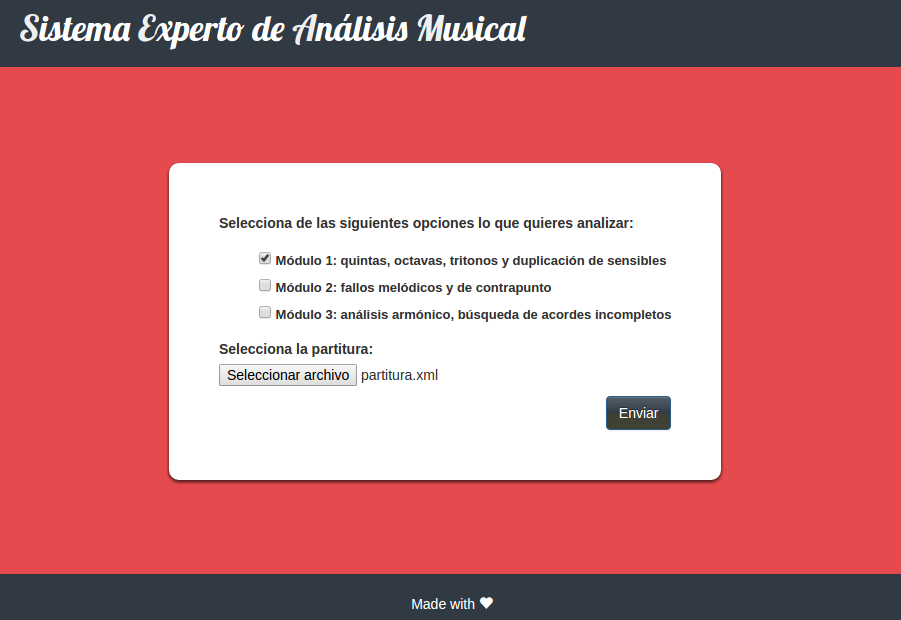
\includegraphics[scale=0.35]{imagenes/interfaz3.png}
	\caption{Página principal}
	\label{fig5.3.1}
\end{figure}

\begin{figure}[H]
	\centering
	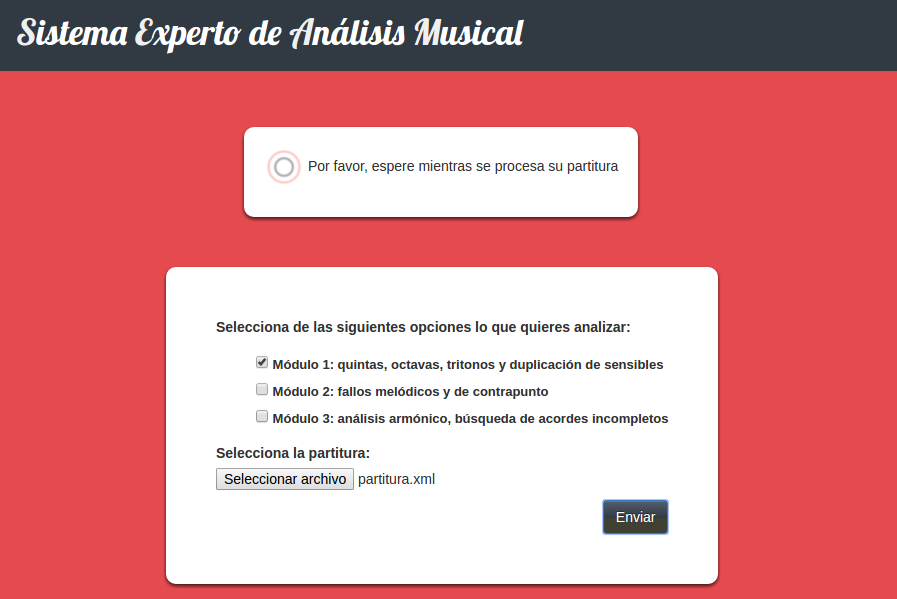
\includegraphics[scale=0.35]{imagenes/interfaz4.png}
	\caption{Página principal tras enviar el formulario}
	\label{fig5.3.2}
\end{figure}

\bigskip

\begin{figure}[H]
	\centering
	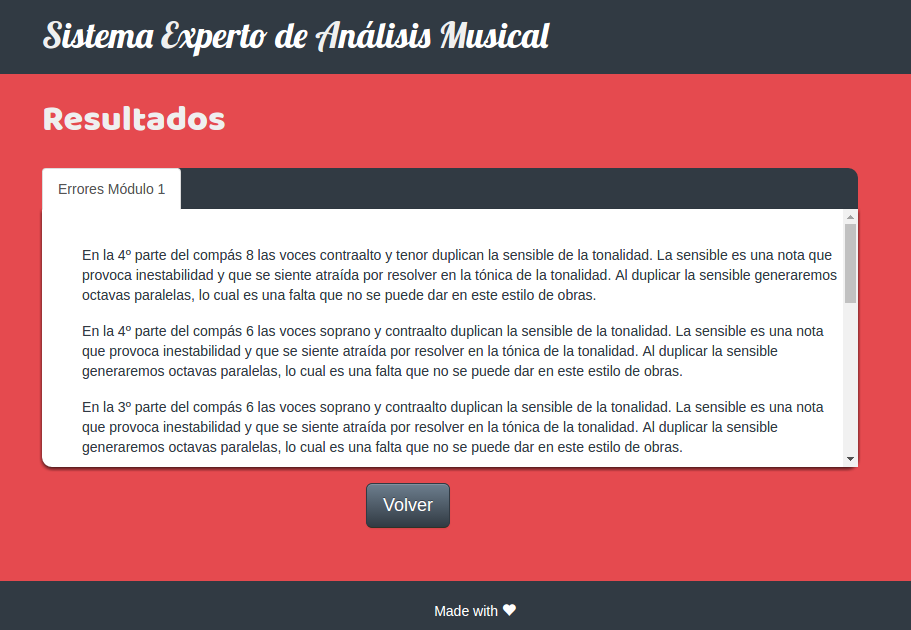
\includegraphics[scale=0.35]{imagenes/interfaz5.png}
	\caption{Visualización de resultados con errores}
	\label{fig5.3.3}
\end{figure}

\begin{figure}[H]
	\centering
	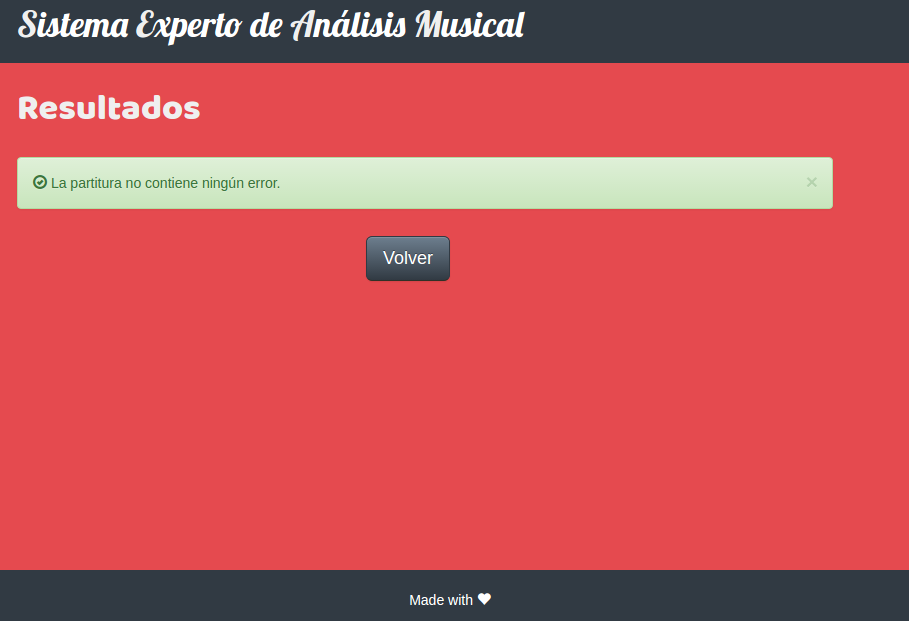
\includegraphics[scale=0.35]{imagenes/interfaz6.png}
	\caption{Visualización de resultados sin errores}
	\label{fig5.3.4}
\end{figure}